\documentclass[class=NCU_thesis, crop=false]{standalone}
\begin{document}

\chapter{背景知識與文獻回顧}
\section{背景知識}

本章節將會介紹本論文所需的背景知識,可以幫助讀者更好地理解本論文提出的論文的概念和出發點,
內容包含:人如何感知彩色影像、大腦皮質的運作、卷積神經網路與以卷積神經網路為基礎的可解釋性深度學習模型。

\subsection{人如何感知彩色影像}

要了解人如何感知色彩我們必須要先了解將彩色影像的這條 Central Visual Pathway 會經過哪些的部位與流程,
根據《 Neuroscience 》 \cite{Purves2004Neuroscience3E}所介紹,
彩色影像在 Central Visual Pathway 會經過的部位總共可以分為三個重要部位:視網膜、外側膝狀體(外膝體,Lateral Geniculate Nucleus)、視覺皮層,
彩色影像從視網膜進入後會送入外膝體,外膝體在收到兩側眼球的資訊後會將不同的資訊平行傳輸至不同的視覺皮層,視覺皮層則負責對這些資訊進行分層的整合與感知。
詳細的Central Visual Pathway 如\cref{fig:Central_Visual_Pathway}

\begin{figure}[H]
  \centering
  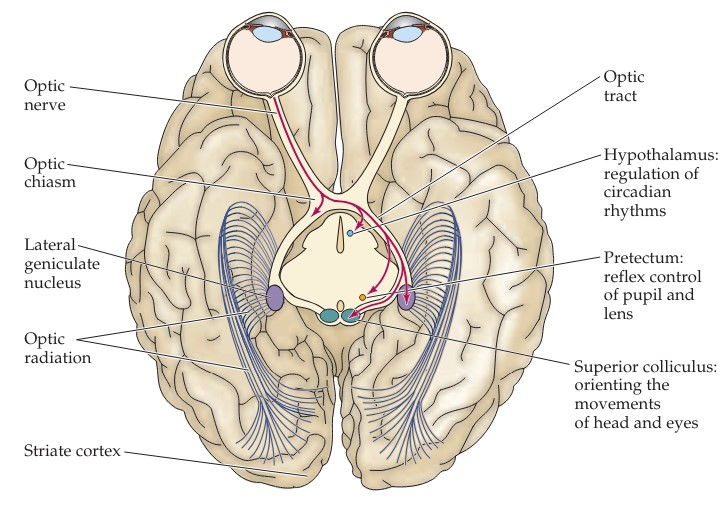
\includegraphics[width=0.7\textwidth]{Central_Visual_Pathway.jpg}
  \caption{詳細視覺路徑圖~\cite{Purves2004Neuroscience3E}}
  \label{fig:Central_Visual_Pathway}
\end{figure}

\subsubsection{視網膜}

外界事物將光反射進入眼睛當中,透過眼珠中的角膜與水晶體等透明的光學介質進行折射最終聚焦於視網膜表面的感光層上形成影像。
在光聚焦於視網膜表層時,視網膜會將光轉換成動作電位並透過視神經傳輸至外膝體,也因此Central Visual Pathway 才會將視網膜視為感知彩色影像的第一個重要部位。

根據《Neuroscience-Exploring the Brain》\cite{bear2016neuroscience}
我們知道視網膜的基礎架構是由五類細胞組成如\cref{fig:RetinaBasic},分別是: 感光細胞、 水平細胞、 無長突細胞、 雙極細胞、 神經節細胞。 感光細胞包含我們常聽到的視錐細胞等負責將輸入的光轉化為動作電位、 雙極細胞負責將會將感光細胞的電位傳送到神經節細胞、
這個傳輸的過程有些則是由水平細胞和無長突細胞協助傳輸,
神經節細胞則負責將最後的資訊傳輸到外膝體之中。

\begin{figure}[H]
  \centering
  \subcaptionbox{
    視網膜基本架構~\cite{bear2016neuroscience}
    \label{fig:RetinaBasic}}
    {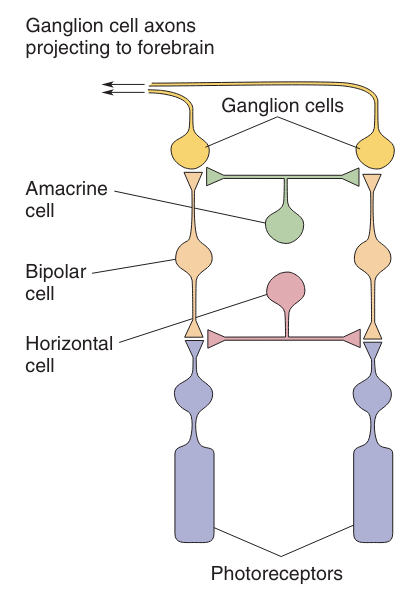
\includegraphics[width=0.5\textwidth]{RetinaBasic.png}
    }
~
  \subcaptionbox{
    視網膜層級架構~\cite{bear2016neuroscience}
    \label{fig:RetinaStructure}
  }
    {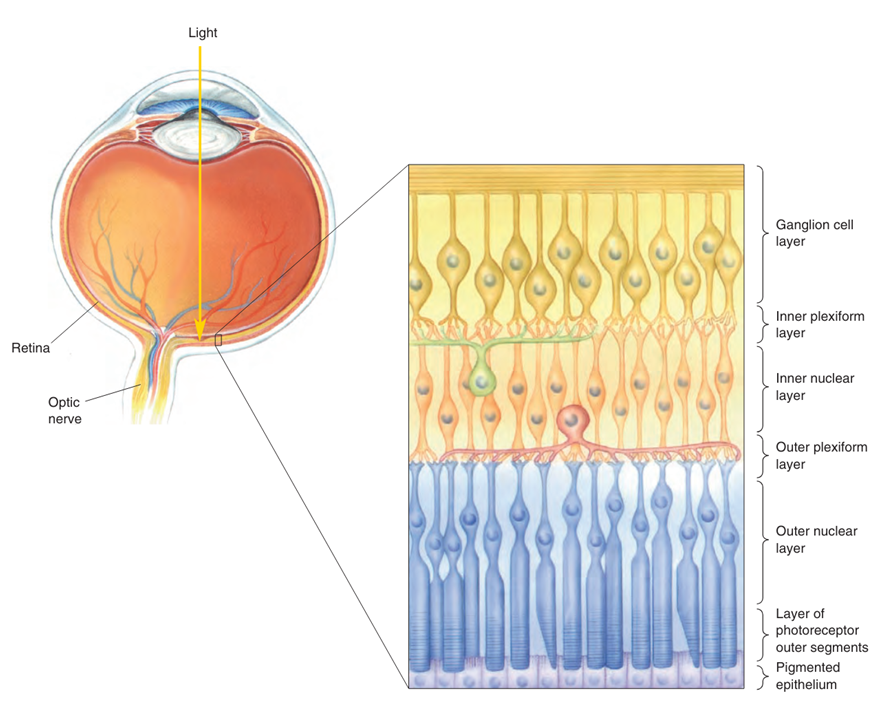
\includegraphics[width=0.9\textwidth]{RetinaStructure.png}
    }
  \caption{視網膜整體架構}
  \label{fig:RetinaTotalStructure}
\end{figure}

上面講的基礎架構只是最基礎的情況,事實上視網膜的各類細胞遠比上面要架構要複雜許多,上述的五大類細胞還可以再更細的分為不同功能的變種細胞,由此組成了極度複雜的視網膜層級系統如\cref{fig:RetinaStructure}。
如此複雜的視網膜系統,其功能當然不只負責影像的感知與電位傳輸,事實上
在2013年的\cite{annurev},就已經發現在感光細胞將光轉換為動作電位後會將電位傳輸到層級架構的 Inner Plexiform Layer(IPL)中不同變種的雙極細胞,這些不同變種的雙極細胞對收到的影像資訊進行不同的平行處理,最終輸出影像中不同的方面的要素到神經節細胞,例如: 紅藍綠不同色彩、明暗的變化、影像輪廓等等, 這同時也是本論文在設計彩色影像感知時的核心概念。

\begin{figure}[H]
  \centering
  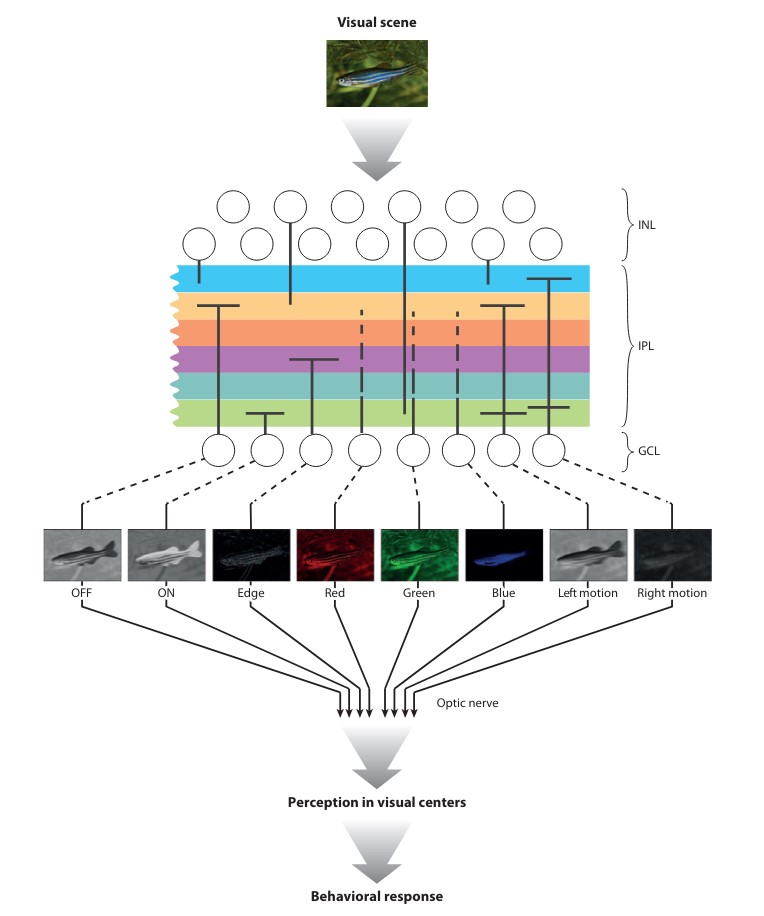
\includegraphics[width=0.7\textwidth]{IPL.jpg}
  \caption{視網膜對影像進行不同的平行處理~\cite{annurev}}
  \label{fig:IPL}
\end{figure}

\subsubsection{外側膝狀體}

外側膝狀體(外膝體)主要負責將視網膜不同的方面資訊(如:色彩、輪廓、運動方向…)傳輸到對應的初級視覺皮質,其中的細胞分層排列,每層分布排列著著不同種類的細胞。
除此之外,外膝體中不同的細胞層也對應著不同視野的半個視網膜形成如 \cref{fig:LGN_Relation}
的對應關係,這也表示視網膜中相鄰區域的同種類的影像資訊在外膝體中很可能在同一個細胞層。
由於視覺皮層會將影像資訊從初級到高級逐漸進行整合和學習但始終維持著資訊的平行,
因此外膝體的存在可以協助視覺皮層將不同的影像資訊傳輸到對應的視覺皮質層,
這對視覺皮質能夠進行平行處理起到至關重要的作用。

\begin{figure}[H]
  \centering
  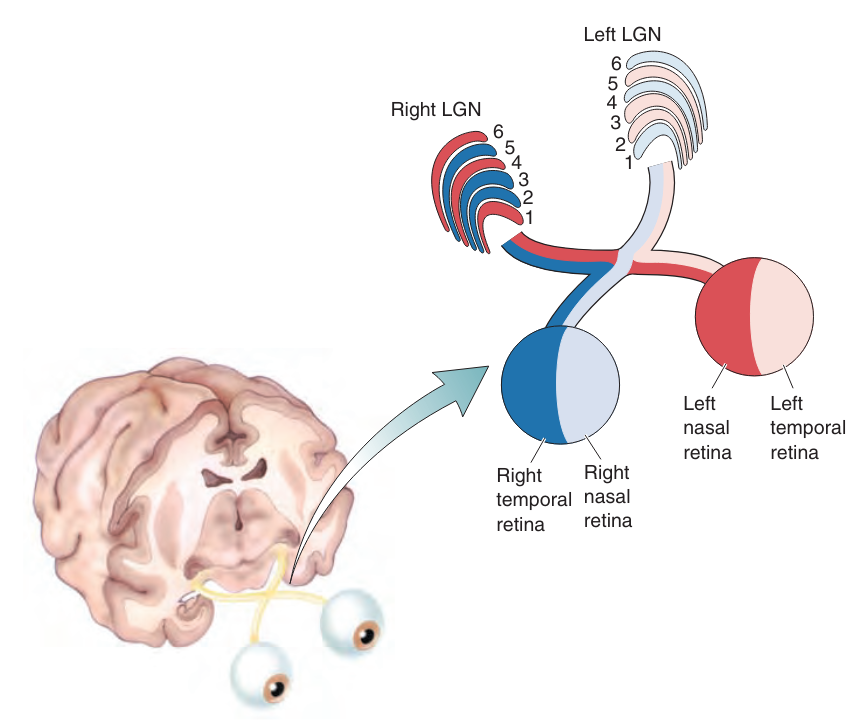
\includegraphics[width=0.7\textwidth]{LGN_relation.png}
  \caption{視網膜與外膝體的對應關係~\cite{bear2016neuroscience}}
  \label{fig:LGN_Relation}
\end{figure}


\subsubsection{視覺皮層}


\subsection{卷積神經網路}

\subsection{以卷積神經網路為基礎的可解釋性深度學習模型}

\section{文獻回顧}

\subsection{可解釋性人工智慧的演進與分類}
Decision Tree:
\cite{rokach2016decision}
\cite{grinsztajn2022treebased}

介紹可解釋性人工智慧的歷程,分類,各分類著名的論文的簡介
可解釋性人工智慧的研究最早可以追蹤到1991年的專家系統時代 W Swartout, C Paris 等人便開始對可解釋性人工智慧進行研究 \cite{87686},
但是

\subsection{對於 Inherently Interpretable 可解釋性模型之研究}
\subsubsection{基於多層自我映射圖之可視覺化深度學習模型}

\subsection{對於 Post-hoc 可解釋性模型之研究}
\subsubsection{Local Interpretable Model-agnostic Explanations(LIME)} 
\subsubsection{Shapley Additive Explanations(SHAP)}

\subsection{近年可解釋性模型趨勢之研究}
\subsubsection{Tabnet: Attentive interpretable tabular learning}
\subsubsection{Building more explainable artificial intelligence with argumentation}
XAI的新趨勢使用論證的方式來解釋,特別是計算論證有助於理解理性決策的所有步驟以及在不確定性下進行推理。 \cite{LONGO2024102301}



\end{document}